%% LyX 2.3.0 created this file.  For more info, see http://www.lyx.org/.
%% Do not edit unless you really know what you are doing.
\documentclass{article}
\usepackage[latin9]{luainputenc}
\usepackage{geometry}
\geometry{verbose}
\usepackage{esint}

\makeatletter
%%%%%%%%%%%%%%%%%%%%%%%%%%%%%% User specified LaTeX commands.

%%%%%%%%%%%%%%%%%%%%%%%%%%%%%%%%%%%%%%%%%%%%%%%%%%%%%%%%%%%%%%%%%%%%%%%%%%%%%%%%%%%%%%%%%%%%%%%%%%%%%%%%%%%%%%%%%%%%%%%%%%%%%%%%%%%%%%%%%%%%%%%%%%%%%%%%%%%%%%%%%%%%%%%%%%%%%%%%%%%%%%%%%%%%%%%%%%%%%%%%%%%%%%%%%%%%%%%%%%%%%%%%%%%%%%%%%%%%%%%%%%%%%%%%%%%%
\usepackage{tikz}




\newtheorem{theorem}{Theorem}\newtheorem{acknowledgement}[theorem]{Acknowledgement}\newtheorem{algorithm}[theorem]{Algorithm}\newtheorem{axiom}[theorem]{Axiom}\newtheorem{case}[theorem]{Case}\newtheorem{claim}[theorem]{Claim}\newtheorem{conclusion}[theorem]{Conclusion}\newtheorem{condition}[theorem]{Condition}\newtheorem{conjecture}[theorem]{Conjecture}\newtheorem{corollary}[theorem]{Corollary}\newtheorem{criterion}[theorem]{Criterion}\newtheorem{definition}[theorem]{Definition}\newtheorem{example}[theorem]{Example}\newtheorem{exercise}[theorem]{Exercise}\newtheorem{lemma}[theorem]{Lemma}\newtheorem{notation}[theorem]{Notation}\newtheorem{problem}[theorem]{Problem}\newtheorem{proposition}[theorem]{Proposition}\newtheorem{remark}[theorem]{Remark}\newtheorem{solution}[theorem]{Solution}\newtheorem{summary}[theorem]{Summary}\newenvironment{proof}[1][Proof]{\noindent\textbf{#1.} }{\ \rule{0.5em}{0.5em}}


\newcommand{\ind}[1]{{\bf 1  }[ #1 ] }

\makeatother

\begin{document}
\begin{center}
\textbf{Econ 512}
\par\end{center}

\begin{center}
\emph{Fall 201}9\\[1em]
\par\end{center}

\begin{center}
Homework 4 -- Numerical Integration \\
 Due 11/04/2019 \\[3em] 
\par\end{center}

\bigskip{}

There are multiple ways to compute the mathematical constant $\pi$
via numerical integration. Probably the simplest is the ``dart-throwing''
method, which is a special case of an \textit{accept-reject} simulator.
A somewhat more elegant approach comes from an integral representation.
This homework will consider both. Consider the quarter-circle arc
of radius 1, centered at the origin inscribed within the unit square:

%\begin{figure}

\begin{center}
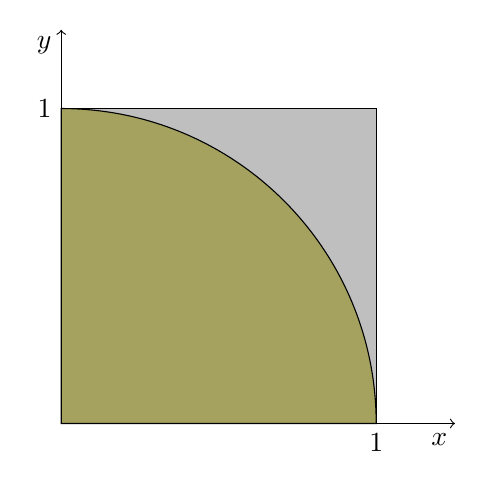
\begin{tikzpicture}[scale = 4]
\draw [<->] (0, 1.25) -- (0,0) -- (1.25, 0);
\draw [fill=lightgray] (0,1) rectangle (1, 0);
\filldraw[fill opacity=0.5,fill=olive] (0,0) -- (1, 0) arc (0:90:1) -- cycle;
\node [below] at (1,0) {$1$};
\node [below] at (1.2,0) {$x$};
\node [left] at (0, 1) {$1$};
\node[left] at (0, 1.2) {$y$};
\end{tikzpicture} %\caption{Unit interval with arc}
\par\end{center}

%\end{figure}

Clearly, the area of the quarter-circle (green shaded area) is $\frac{\pi}{4}$
whereas the area of the unit square is 1. For any point inside the
unit square, we can tell whether it lies within the quarter-circle
using the Pythagorean formula. That is, $(x,y)$ lies within the shaded
are if $x^{2}+y^{2}\leq1$. The dart-throwing method simply draws
points uniformly from within the unit square and accepts them when
they lie within the circle and rejects them otherwise. The ratio of
acceptances to total draws converges to the area of the quarter circle.
In other words, we can calculate $\pi$ using the double-integral,

\[
\pi=4\int_{0}^{1}\int_{0}^{1}\ind{x^{2}+y^{2}\leq1}dydx.
\]

\begin{enumerate}
\item Write an algorithm that uses the dart-throwing method to approximate
$\pi$ using a quasi-Monte Carlo approach to computing integrals.
\item Write an algorithm that uses the dart-throwing method to approximate
$\pi$ using a Newton-Cotes approach to computing integrals.
\end{enumerate}
However, all we are doing is calculating the area under the curve.
From the same figure and again using Pythagorean formula, one can
solve for $y$ as a function of $x$, $y=\sqrt{1-x^{2}}$. Thus, we
have a definition for $\pi$ based on a single dimensional integral,

\[
\pi=4\int_{0}^{1}\sqrt{1-x^{2}}dx.
\]

\setcounter{enumi}{2} 
\begin{enumerate}
\item Approximate $\pi$ based on the above integral using a quasi-Monte
Carlo approach.
\item Approximate $\pi$ based on the above integral using a Newton-Coates
approach.
\item Prepare a table which shows the mean squared error of 200 simulations
if pseudo-MC integration using 100, 1000 and 10,000 draws. Compare
this to the squared error of the quasi-MC and Newton-Coates methods
for the same number of quadrature draws (i.e., nodes).
\end{enumerate}

\end{document}
